\section{Evaluation}
\label{idea-sec-evaluation}

To evaluate IDEA, we build and test the two energy-aware components and
one energy-aware application described in Section~\ref{idea-sec-casestudies}. For
the LPL tuning and routing components, we compare the performance of our
IDEA-based implementations to approaches that are not energy-aware.
For the third application, we use IDEA to implement several energy objective
functions and compare their performance against each other and against a
heuristic that does not consider energy availability.

\subsection{Experimental Setup}
\label{idea-subsec-experimentalsetup}

Throughout the evaluation we present results run in several different
environments. We have implemented IDEA for TinyOS in order to run experiments
on MoteLab~\cite{motelab}, our 180~node wireless sensor network testbed
located across three floors of an office building. We also present results
obtained using TOSSIM~\cite{tossim}, the TinyOS simulator.  TOSSIM
incorporates a closest-fit pattern matching noise model to accurately capture
complex link dynamics~\cite{cpm-ipsn07}. TOSSIM allows us to run longer
experiments incorporating various solar charging models. To improve the
realism of TOSSIM we began with a modified version developed for the Koala
project~\cite{koala-ipsn08} and performed further modifications to correctly
simulate the operation of LPL. We use information collected on MoteLab to
build a realistic TOSSIM radio model for our simulations.  Finally, for the
third application we built a Python simulator to allow rapid prototyping of
various energy objective functions.

IDEA is designed to tune components in the face of variations in both load
and charging rates, and to test this we present experiments using solar
charging data collected off of a solar panel deployed on a Enfield, MA
rooftop in March, 2009. Battery levels are calculated using a charging model
based on a Nickel-Metal Hydride battery technology with a 66\% charging
efficiency. We attenuate this data to simulate the charging produced by solar
panels of several different sizes in order to evaluate IDEA's performance as
available energy changes. We also perform experiments with a randomly
attenuated charging profile to simulate the effects of bad solar panel
placement or obstacles to incident sunlight that could effect the spatial
distribution of collected energy.

For our MoteLab experiments we determine the system's ability to span periods
without charging inputs. We use two sets of initial conditions designed
around our observations of the interaction between the charging data we
collected and the capacity of the batteries deployed. If the solar panel is
large enough it will provide considerable charging input and completely
charge small batteries during the day. For this scenario all nodes begin the
night with full batteries and are trying to last until sunrise. If the solar
panel is not large enough to completely charge the batteries nodes will begin
the night with varying amounts of charge depending on their load rates during
the day.

Energy tracking is done by IDEA using a software-only approach developed for
the Pixie~\cite{pixie-sensys08} project. The component captures state
transitions and applies an energy consumption model for each state based on
current consumption measured offline. In the future we would like to
integrate a more accurate hardware-driven approach such as
iCount~\cite{icount-spots08}. The short lifetimes for some experiments are
explained by the use of extremely small batteries, which were chosen to allow
experiments to complete in reasonable amounts of time. We expect that
application developers will want to use a battery size and charging
technology suitable to allow their system to achieve a desired level of
performance, and the improvements in energy efficiency possible using IDEA
will allow smaller batteries or solar panels to be used, reducing the size
and cost of the hardware package.

Experiments for the LPL tuning and energy-aware routing cases use the
first-node death energy objective function described in
Section~\ref{idea-subsec-energyobjectivefunctions}, and therefor we evaluate the
network lifetime as the time at which the first node runs out of energy. Our
distributed localization application illustrates the process of designing an
effective energy objective function when the overall goal of the system is
known.

\subsection{LPL parameter tuning}
\label{idea-subsec-lplparametertuning}

\begin{figure}[t]
\label{idea-table-lplvoptimalmotelab}
\begin{center}
\begin{tabular}{|l|ccc|}
\hline
\textbf{Initial Battery} & \multicolumn{2}{c}{\textbf{Lifetime (hours)}} & \textbf{Increase} \\
\textbf{Levels} & \textbf{Static} & \textbf{Tuned} & \textbf{(\%)} \\ \hline
Uniform & 4.6 & 5.6 & 22\\
Random & 2.8 & 3.0 & 7 \\ \hline
\end{tabular}
\end{center}
\caption{\textbf{LPL tuning performance on MoteLab.}
The table shows results for MoteLab experiments comparing the performance of
the IDEA-driven LPL tuning component against the best static parameter
solution. IDEA shows gains for both the case where all nodes start with the
same battery level and randomly initialized battery states.}
\end{figure}

We begin by evaluating the IDEA-driven LPL parameter tuning component
described in Section~\ref{idea-subsec-lpltuning}.
Figure~\ref{idea-table-lplvoptimalmotelab} summarizes the results of experiments
conducted on a 20~node subset of the MoteLab sensor network testbed. We
configure the nodes into a collection tree with each node sending messages to
the sink once every 2 minutes. As a point of comparison we ran experiments
using static intervals assigned a priori, with all nodes using the same LPL
interval.  We compared the results from all six intervals and picked the one
that performed the best. Note that this experimentation itself is a form of
tuning and would be difficult to do beforehand. We ran one hour testbed
experiments and used each node's rate of energy consumption to compute a
projected lifetime.

The table shows that the tuned LPL intervals produce improvements in
projected lifetimes when compared with the best static interval under both
non-charging scenarios discussed in Section~\ref{idea-subsec-experimentalsetup}.
We observe an improvement of 22\% for the case where nodes start with the
same initial charge and 7\% when random initial battery levels are used. This
is despite the fact that the LPL tuning component produces significant
overhead propagating new state early in the experiment as nodes are moving
from their initial states into their IDEA-tuned intervals.

\begin{figure}[t]
\label{idea-table-lplvoptimaltossim}
\begin{center}
\begin{tabular}{|l|cccc|}
\hline
\textbf{Solar Charging} & \multicolumn{3}{c}{\textbf{Lifetime (hours)}} &
\textbf{Increase} \\
\textbf{Pattern} & \textbf{Static} & \textbf{Tuned} & \textbf{No Overhead} & \textbf{(\%)} \\ \hline
Large Panel & 22.7 & 23.8 & 24.0 & 5\% \\
Small Panel & 16.8 & 18.9 & 21.2 & 13\% \\
Randomly & \multirow{2}{*}{13.8} & \multirow{2}{*}{18.6} & \multirow{2}{*}{20.4} & \multirow{2}{*}{35\%} \\
Attenuated & & & & \\ \hline
\end{tabular}
\end{center}
\caption{\textbf{LPL tuning performance with solar charging.}
This table displays results for TOSSIM experiments comparing IDEA-based LPL
parameter tuning with the best static interval and an overhead-free version
of IDEA. IDEA shows gains over the non-tuned approaches across a range of
different solar charging profiles.}
\end{figure}

Figure~\ref{idea-table-lplvoptimaltossim} summarizes results from experiments
performed on TOSSIM that include solar charging inputs discussed above.  IDEA
provides 5\% and 10\% performance improvements for cases in which all nodes
see the same input charging profile and a 35\% improvement in the case where
charging inputs are randomly attenuated. We believe that this is due to the
increased difference in battery levels due to the random attenuation, which
creates more diversity in the amount of available charge. The table also
shows numbers that indicate the best that IDEA can do when its overhead is
artificially eliminated, showing that future work on improving the load and
charge modeling and more efficient state sharing will continue to improve
performance.

\begin{figure}[t]
\label{idea-fig-lpltopology}
\begin{center}
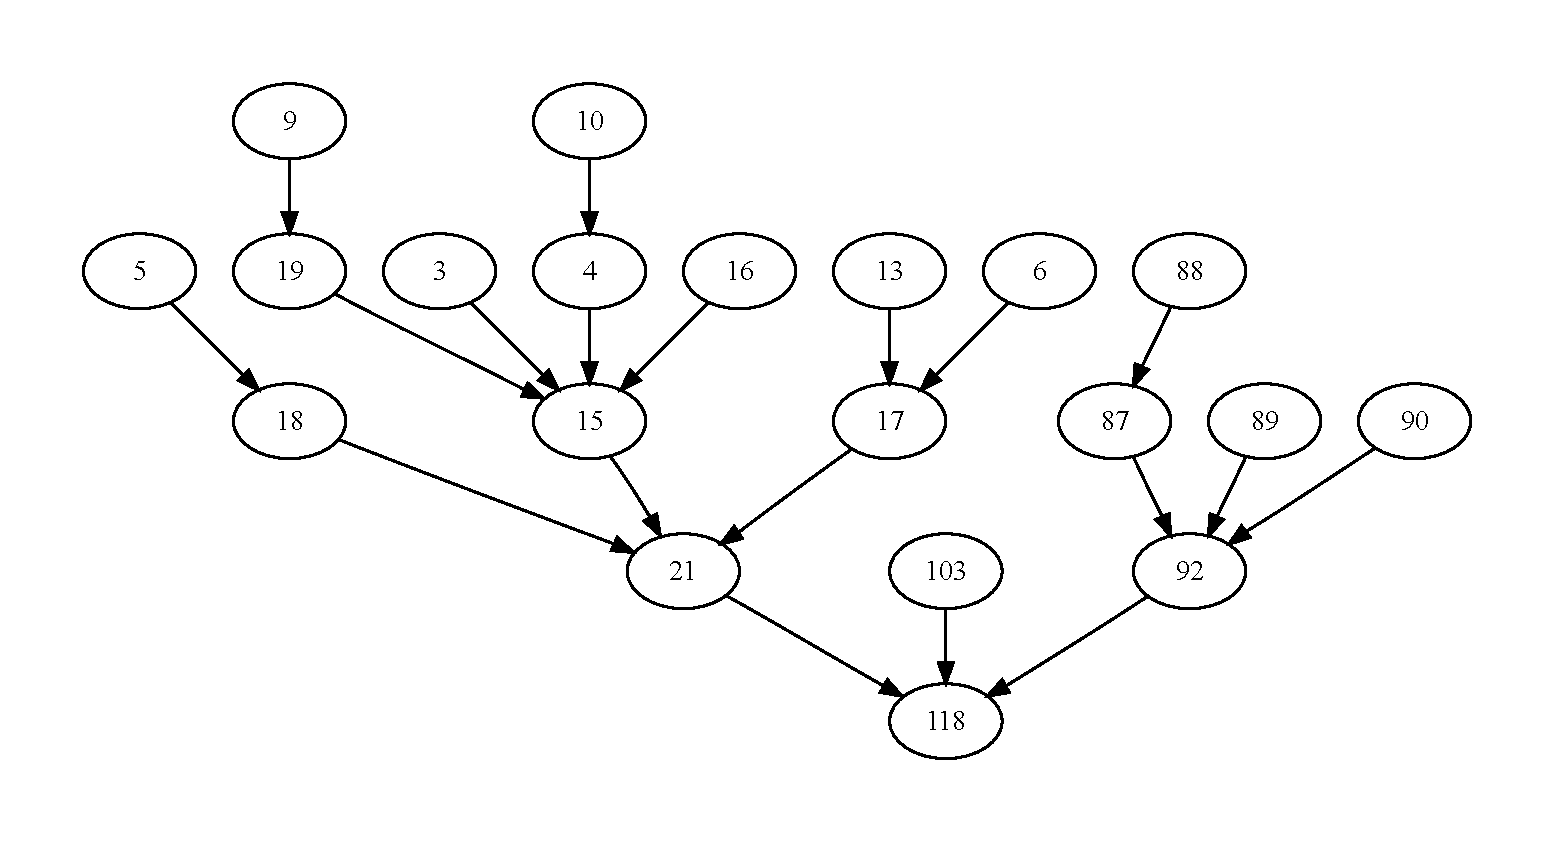
\includegraphics[width=\hsize]{./5-idea/figs/lpltune_topology.pdf}
\end{center}
\caption{\textbf{Topology used for LPL tuning experiments.}}
\end{figure}

\begin{figure}[t]
\label{idea-fig-intervalvoptimal}
\begin{center}
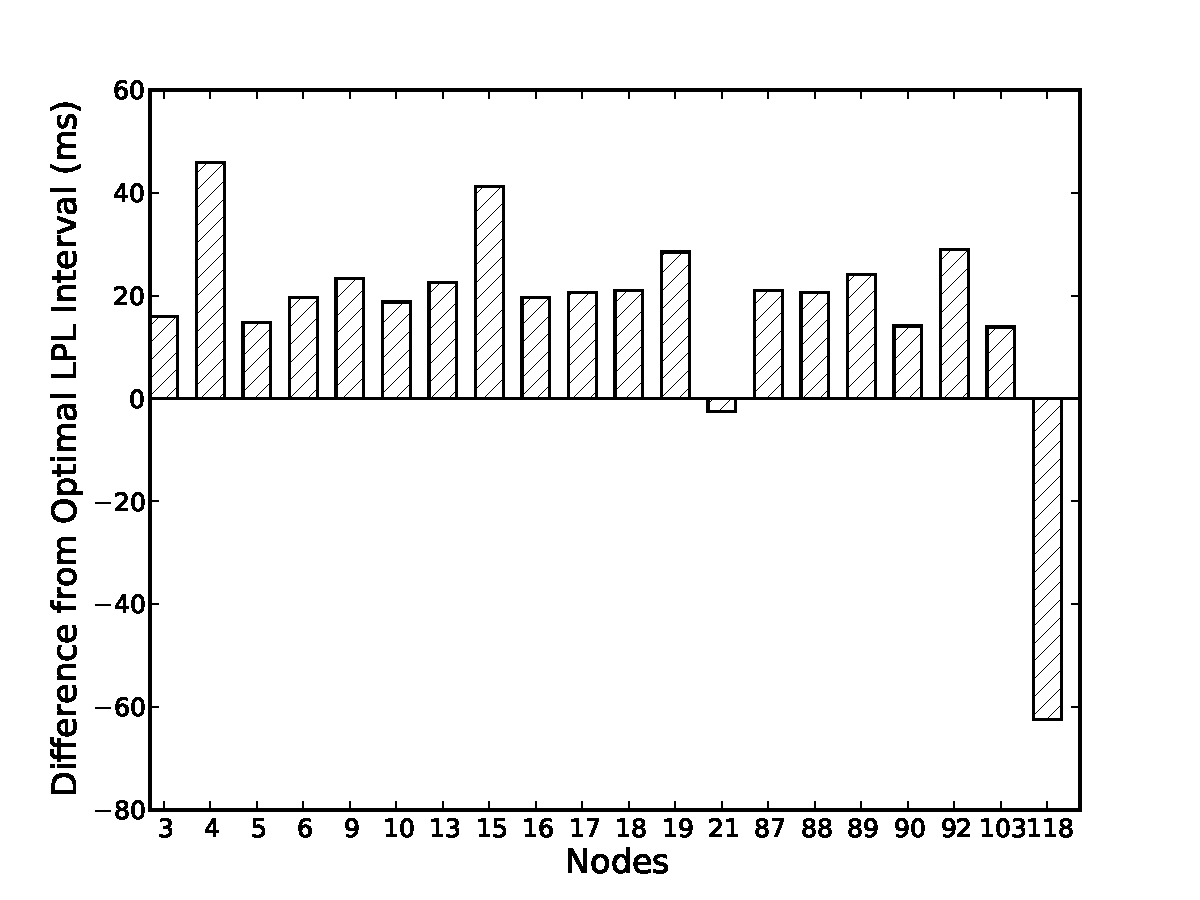
\includegraphics[width=\hsize]{./5-idea/figs/graph_lpl_interval_comparison.pdf}
\end{center}
\caption{\textbf{LPL interval comparison with optimal.}
To assess the degree to which the IDEA-driven approach finds a near optimal
global state we plot difference (in ms) between the intervals chosen by the
IDEA-tuned and offline optimal systems.  The plot demonstrates that IDEA sets
the LPL intervals of nodes similarly to the optimal solution and helps
explain its performance.}
\end{figure}

In the non-charging case we can produce an offline-optimal estimate of the
possible performance by treating the problem as a multi-dimensional,
multiple-choice knapsack problem and computing a solution. We use the optimal
solution as a qualitative point of comparison in
Figure~\ref{idea-fig-intervalvoptimal}, which shows the differences between
intervals picked by the IDEA-driven and optimal solutions for a non-charging
TOSSIM experiment using a 20~node tree, shown in
Figure~\ref{idea-fig-lpltopology}. Most nodes are leaf nodes and correctly choose
the maximum interval possible, and IDEA chooses near-optimal intervals for
Node 21, the energy bottleneck (within 1\% of optimal), and Node 118, the
sink (within 15\% of optimal).

\begin{figure}[t]
\label{idea-fig-lploverhead}
\begin{center}
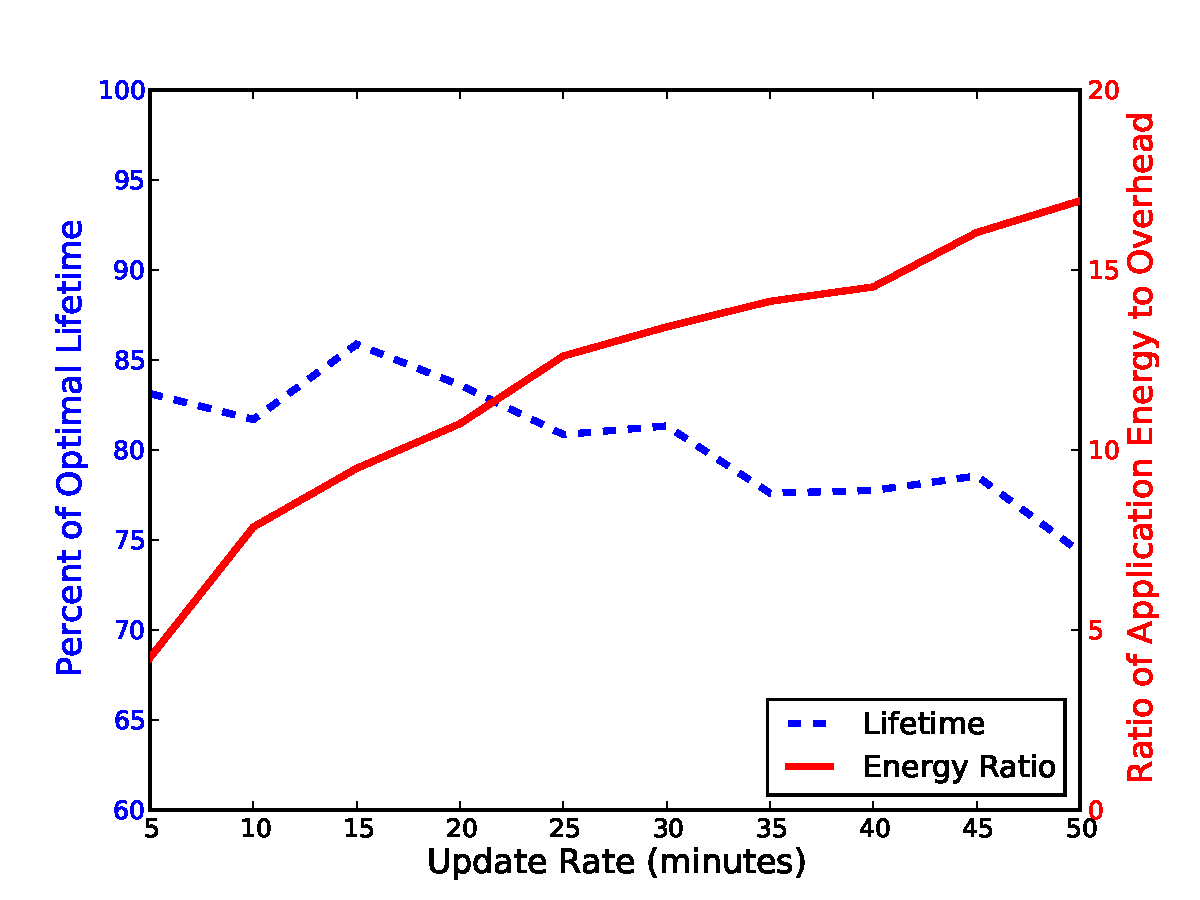
\includegraphics[width=\hsize]{./5-idea/figs/graph_update_rate_overhead.pdf}
\end{center}
\caption{\textbf{Optimality vs. overhead.}
IDEA consumes energy in order to propagate load and charge information. For
the LPL-tuning component the rate of energy overhead is related to the rate
at which we retune the local LPL interval. This plot shows both the IDEA
overhead and the degree of optimality achieved as the tuning rate is
varied.}
\end{figure}

We also use the optimal results to examine the impact of the overhead of the
IDEA LPL-tuning component as we vary the rate at which it selects new
intervals. The update rate determines the number of broadcast messages
generated by nodes as they change their intervals.
Figure~\ref{idea-fig-lploverhead} shows the variation in lifetime, plotted as
percent of the optimal solution, and the energy ratio calculated as the
number of useful joules divided by the number of joules consumed by IDEA in
the form of state sharing. As we decrease the update rate the tuning
component changes state less frequently and consumes less power, causing the
energy ratio to increase. The lifetime curve shows a sweet spot at an update
rate of 15 minutes. At the left end of the curve with a rapid update rate the
overheads associated with state sharing reduce the systems lifetime, and at
the right end of the curve the system is slow to find the optimal state and
the lifetime again suffers.  Across the entire range, however, the achieved
network lifetime remains above 74\% of the optimal offline solution.

%\begin{figure}[t]
%\begin{center}
%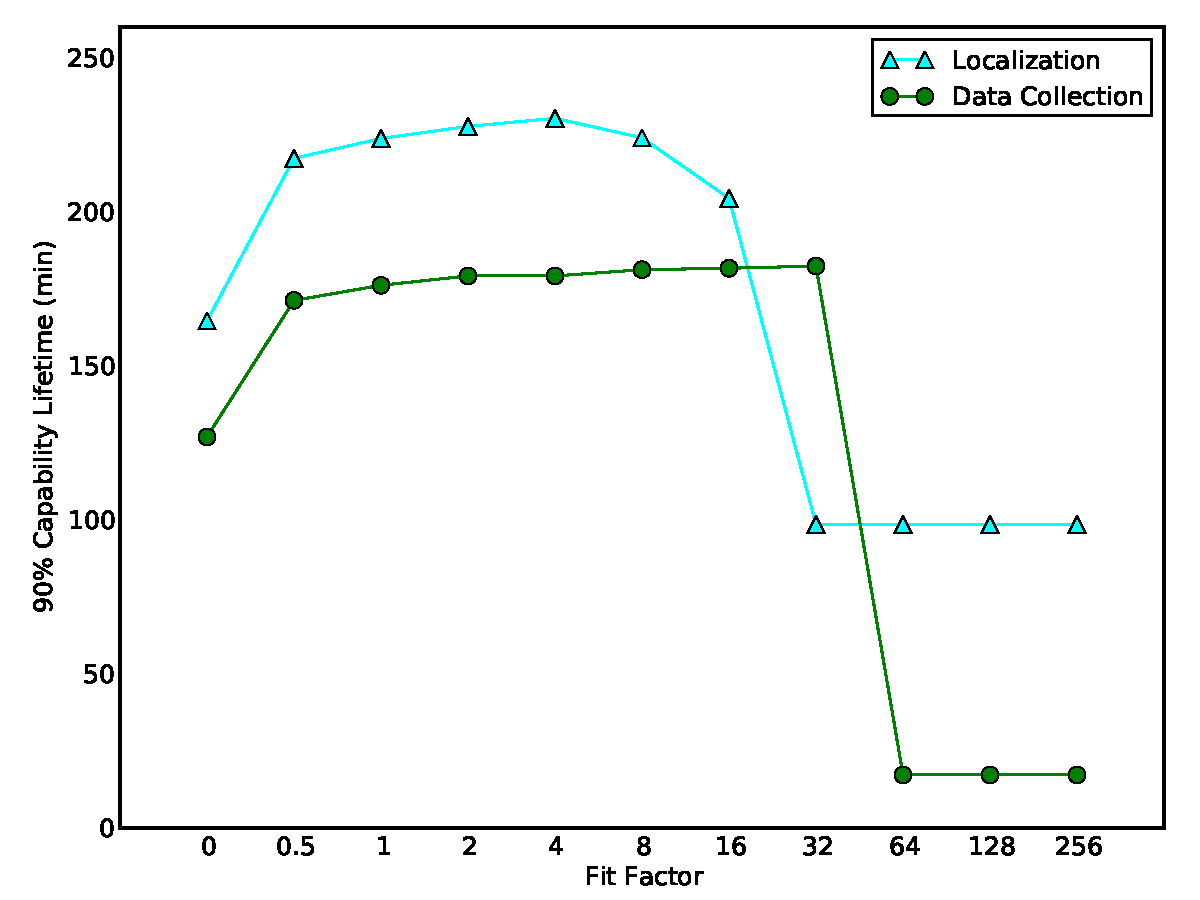
\includegraphics[width=\hsize]{./5-idea/figs/Placeholder.pdf}
%\end{center}
%\caption{\small{\textbf{Testbed comparison with optimal and static intervals.}
%\XXXnote{GWA: A lot of this text should be moved to the discussion and out of
%the caption.}
%Comparing the performance of the IDEA-driven LPL tuning component against
%both an offline-optimal solution and a static parameter solution shows how
%IDEA improves on the static solution, achieving a \XXXnote{FIXME}\% increase
%in lifetime and achieving \XXXnote{FIXME}\% of the lifetime of the offline optimal,
%overhead free solution. \XXXnote{GWA: Need to expand caption if we run
%experiments with overhead-free state sharing.}}}
%\label{idea-fig-lplvoptimalmotelab}
%\end{figure}

%\begin{figure}[t]
%\begin{center}
%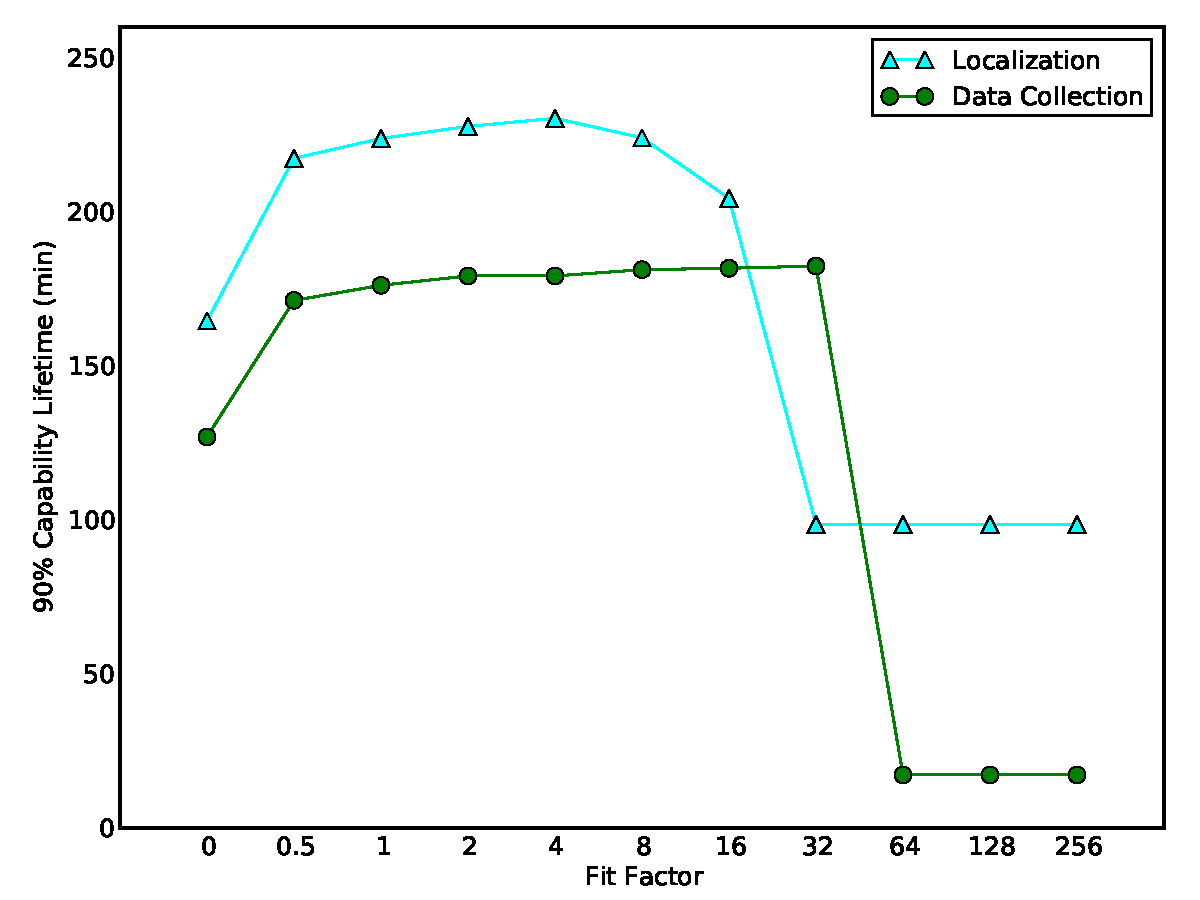
\includegraphics[width=\hsize]{./5-idea/figs/Placeholder.pdf}
%\end{center}
%\caption{\small{\textbf{TOSSIM comparison with optimal and static intervals
%including charging inputs.}
%\XXXnote{GWA: A lot of this text should be moved to the discussion and out of
%the caption.}
%Similar to Figure~\ref{idea-fig-lplvoptimalmotelab}, this figure shows results for
%another set of experiments comparing IDEA-based LPL parameter tuning with a
%piecewise-optimal offline solution and the best static interval. IDEA shows
%similar gains over non-tuned approaches across a range of different solar
%charging profiles.}}
%\label{idea-fig-lplvoptimaltossim}
%\end{figure}


\subsection{ICTP: Energy aware routing}

\begin{figure}[t]
\label{idea-fig-ictpqualitative}
\begin{center}
\textbf{(a)}\\
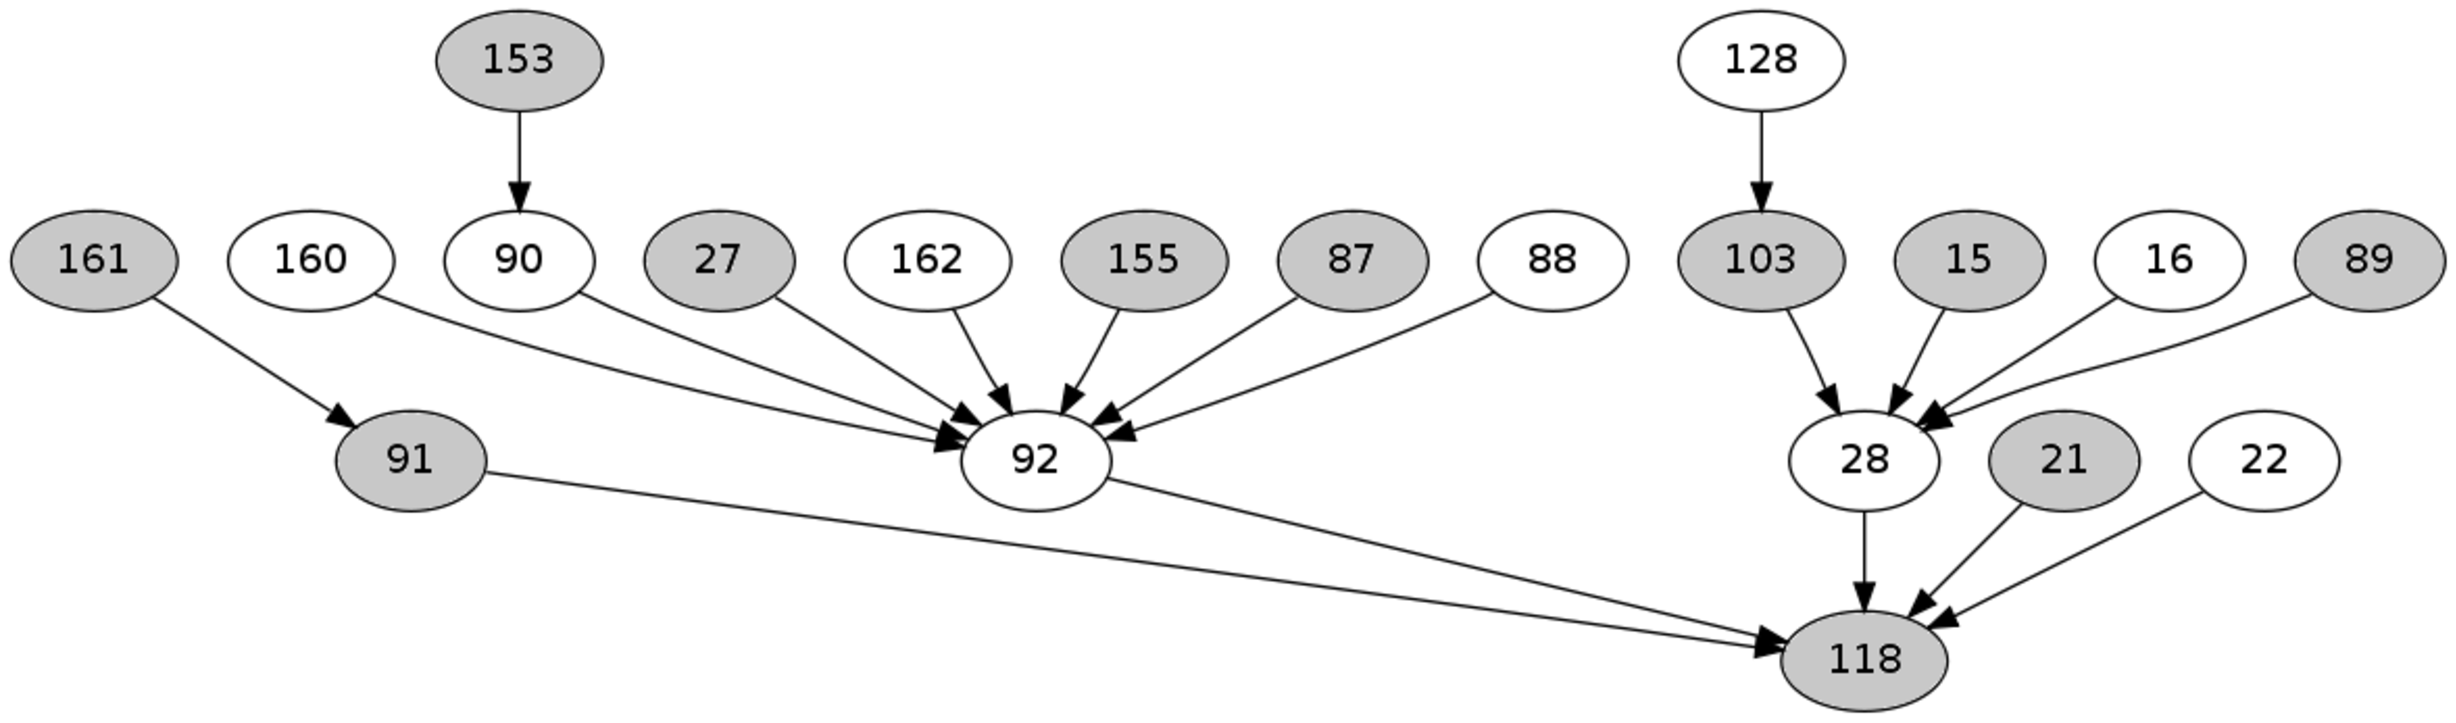
\includegraphics[width=\hsize]{./5-idea/figs/STOCK.pdf}\\
\textbf{(b)}\\
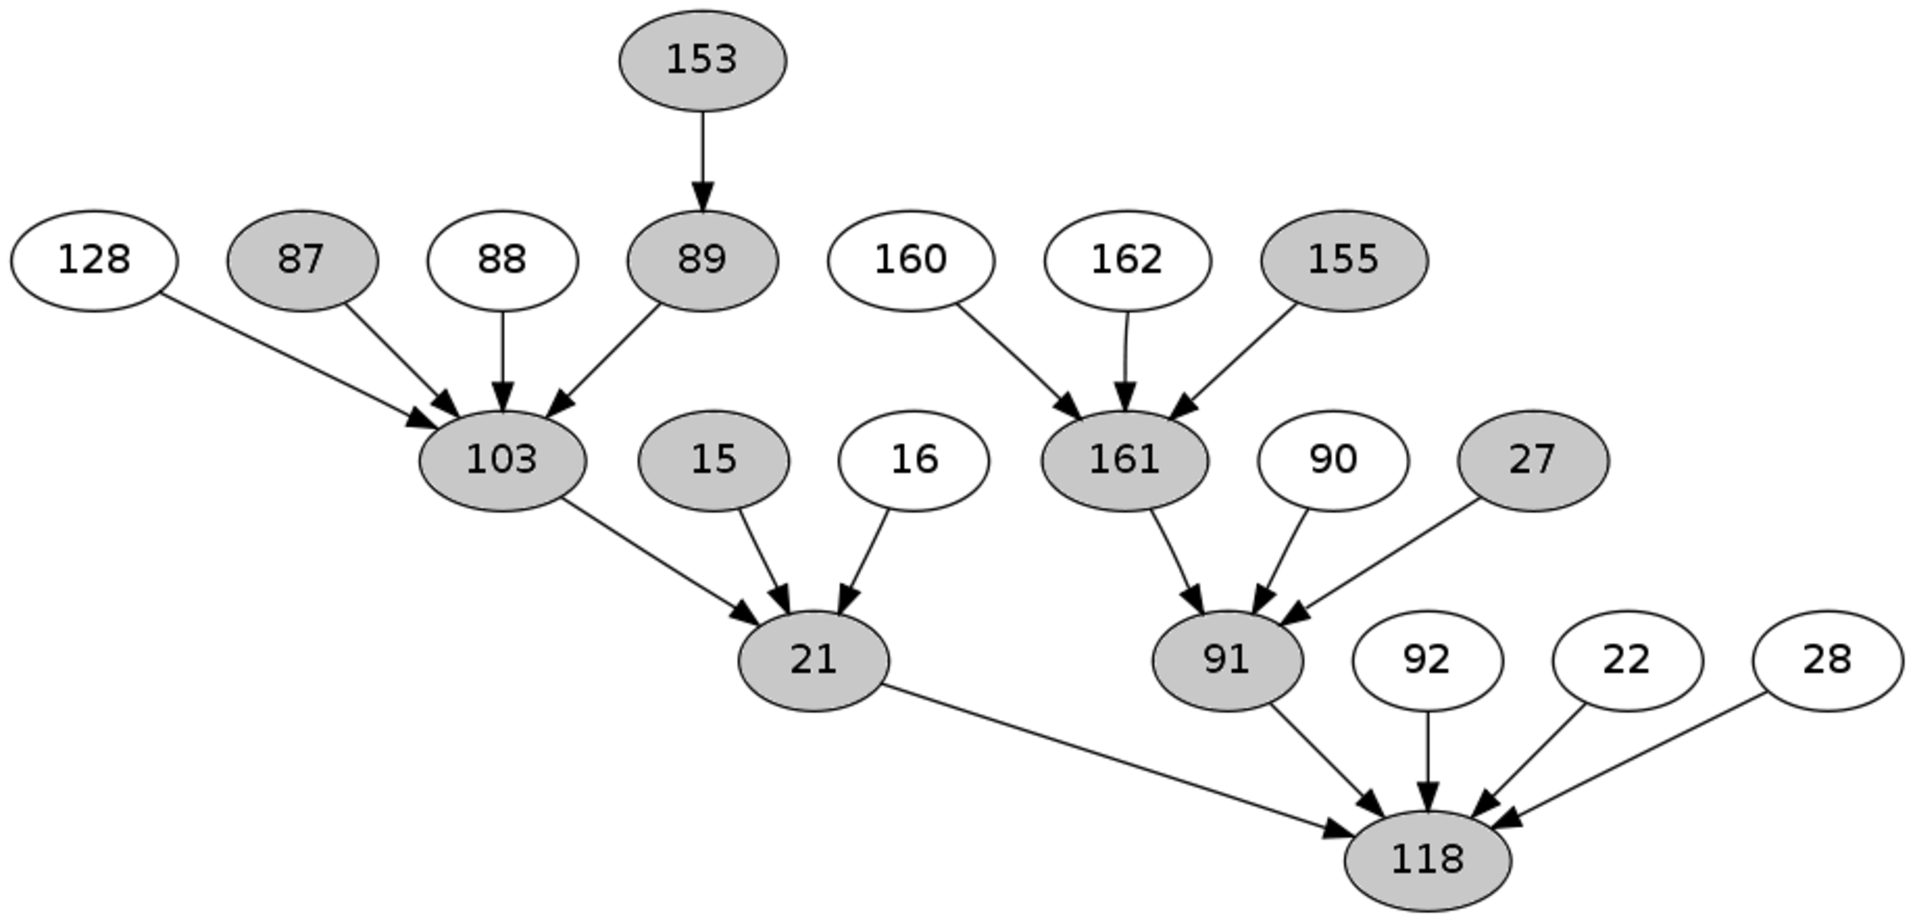
\includegraphics[width=\hsize]{./5-idea/figs/ICTP.pdf}\\
\end{center}
\caption{\textbf{Qualitative comparison of stock CTP and ICTP.}
For this experiment odd-numbered nodes (shaded) were set to charging rapidly,
while even-numbered nodes were not charging. Unmodified CTP builds the tree
shown in (a), which routes many packets through the even nodes. ICTP builds
the tree shown in (b), which moves all even nodes to leaf roles.}
\end{figure}

Using IDEA we were able to integrate energy awareness into CTP, the routing
protocol included as part of TinyOS. For these experiments each node in a
20~node network is sending packets to the sink at the rate of 6 packets per
second. Static LPL intervals of 0.5 second were used. 

Figure~\ref{idea-fig-ictpqualitative} shows a qualitative demonstration of the
differences between energy-aware and non-energy-aware routing trees. This
TOSSIM simulation ran with all odd numbered nodes charging rapidly and all
even numbered nodes not charging (with the exception of the sink, Node 118,
which we assume is powered).  While this is an unrealistic charging pattern,
it produces a clear difference in the routing protocol behavior.
Figure~\ref{idea-fig-ictpqualitative}(a) shows that unmodified CTP is unaware of
these charging differences and puts several even nodes, such as Node 92, into
positions in the routing tree where they are routing for multiple nodes. The
total number of nodes upstream from even numbered nodes in the stock CTP case
is 14. In contrast, ICTP realizes that the odd-numbered nodes have energy to
spare and the even-numbered nodes are lacking, and moves all even nodes into
leaf roles. No even node in Figure~\ref{idea-fig-ictpqualitative} is routing data
for any of its neighbors.

Using a setup similar to that described in
Section~\ref{idea-subsec-lplparametertuning}, we compared the performance of ICTP
to unmodified CTP using 24-hour TOSSIM simulations and the three different
solar charging scenarios previously described. As
Table~\ref{idea-table-lplvoptimaltossim} shows, ICTP shows improvements in
lifetime over stock CTP of between 11 and 27\%. The different routing trees
formed by ICTP did not effect the packet delivery rates appreciably with the
largest change in packet delivery rate with respect to stock CTP being 2.8\%
(97.8\% for CTP vs. 95.0\% for ICTP).

\begin{figure}[t]
\label{idea-table-ictpvoptimaltossim}
\begin{center}
\begin{tabular}{|l|ccc|}
\hline
\textbf{Solar Charging} & \multicolumn{2}{c}{\textbf{Lifetime (hours)}} & \textbf{Increase} \\
\textbf{Pattern} & \textbf{CTP} & \textbf{ICTP} & \textbf{(\%)} \\ \hline
Large Panel & 17.1 & 19.0 & 11\% \\
Small Panel & 10.5 & 13.3 & 27\% \\
Random Attenuation & 10.5 & 12.2 & 16\% \\ \hline
\end{tabular}
\end{center}
\caption{\textbf{ICTP performance with solar charging.}
The table summarizes the improvements in performance obtained by replacing
CTP with ICTP. Three different solar charging profiles are used corresponding
to a large panel that completely charges all batteries during the day, a
small panel that does not completely charge all batteries during the day, and
a randomly attenuated charging profile that varies node-to-node.}
\end{figure}

\subsection{Distributed Localization}

To evaluate the distributed localization application we built a Python
simulator, which improves significantly on TOSSIM performance at this scale
and allowed rapid iteration and experimentation with different energy
objective functions. Our simulator models acoustic event sources within the
sensor network, each of which triggers a distributed localization operation.
The energy overheads of communication, both the leader election process and
the subsequent data transfer, are modeled in the simulator based on empirical
measurements taken on our MoteLab testbed.

\begin{figure}[t]
\label{idea-fig-localizationdensityvtime}
\begin{center}
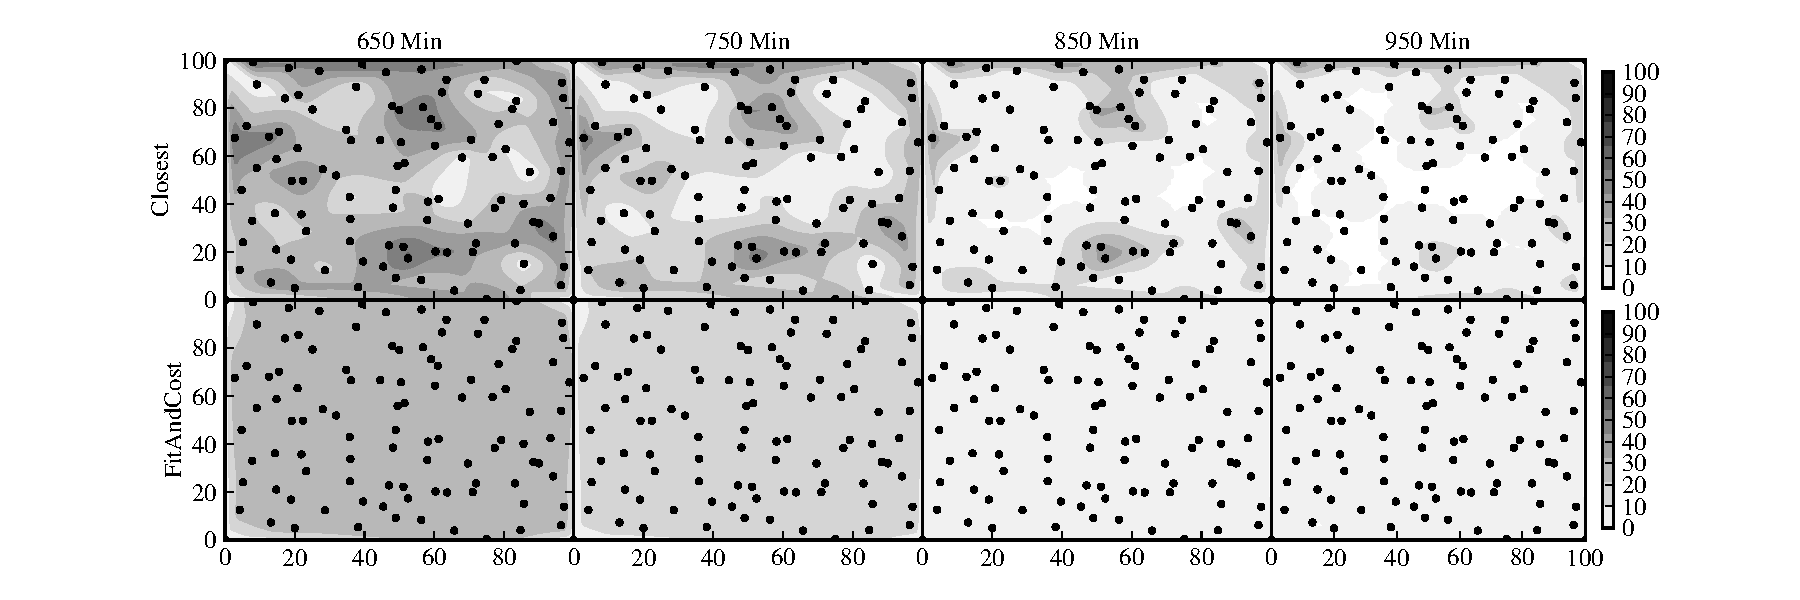
\includegraphics[width=\hsize]{./5-idea/figs/graph_density_vs_time0406_2151.pdf}
\end{center}
\caption{\textbf{Energy density over time.}
Energy densities for the \texttt{Closest} heuristic and IDEA using the
\texttt{WeightedEnergy} objective function are shown at four points in time.
The event distribution is uniform. IDEA enables better load distribution,
which leads to a longer application lifetime.}
\end{figure}

For these experiments we arranged 100 nodes into a 100~m by 100~m area,
resulting in the placements shown in
Figure~\ref{idea-fig-localizationdensityvtime}. We simulate a sensing range equal
to the communication range, each set to 20~m, and randomize the reliable
transfer protocol bandwidth across each link to between 768 and
1280~bytes/sec, a feasible range based on results from data transfer
protocols such as Flush~\cite{flush-sensys07} and
Fetch~\cite{volcano-osdi06}.  Events are simulated using a uniform random
distribution so that events have equal probability of occurring anywhere in
the sensor field.

To evaluate network performance, we define {\em capability} of the network as
the percent of the last 100 operations that succeeded, where success is
defined as localizing the event. We assume that the application requires that
the network be able to localize 90\% of events that occur, and design our
energy objective functions with this in mind. We quote the system lifetime as
the the 90\% capability time, that is the time at which the network's
capability drops below 90\%.

We experimented with several approaches to choosing a localization plan, one
that does not use IDEA and three that do using different energy objective
functions:
\begin{enumerate}
\item \textbf{\texttt{Closest}:} produces a localization plan with the
node closest to the event source as the aggregator and the next three closest
nodes as signal providers. We assume a real solution would use an imperfect
estimate of proximity such as total signal energy or signal-to-noise ratio,
but for the simulations we use the known simulated event location to choose
the closest nodes. \texttt{Closest} does not require energy state information
and so could be implemented without IDEA. It is implemented as an example of
a plausible non-energy-aware solution.
\item \textbf{\texttt{MaxEnergy}:} chooses the node with the most energy
(that heard the event) as aggregator and the next three highest-energy nodes
as signal providers.
\item \textbf{\texttt{TotalEnergy}:} chooses the localization plan that
consumes the lowest amount of total energy summed across all nodes in the
network.
\item \textbf{\texttt{WeightedEnergy}:} weights the total energy consumption
using a similarity metric derived from the cosine similarity index to measure
the degree to which the energy vector for the localization plan is a good
``fit'' given the current energy availability.
\end{enumerate}

\begin{figure}[t]
\label{idea-fig-ideavsheuristics}
\begin{center}
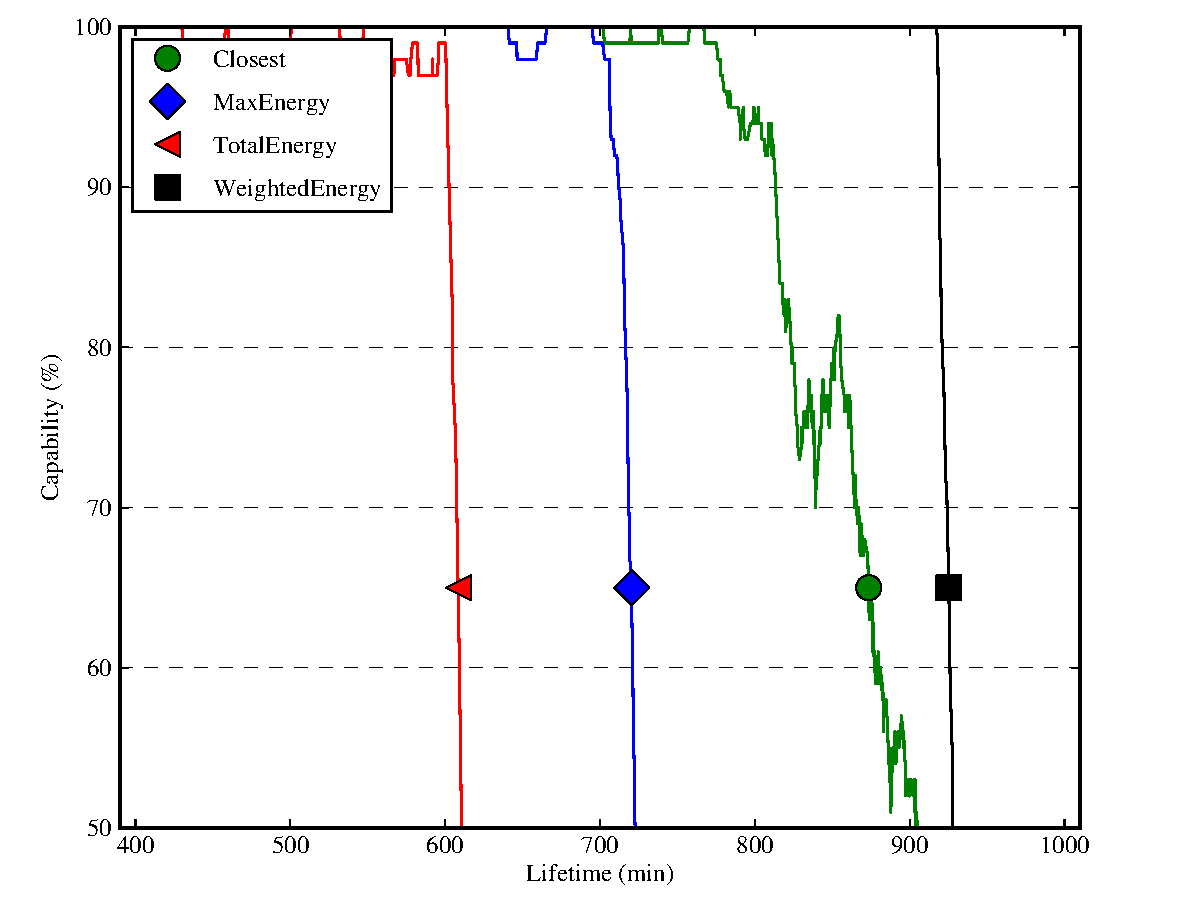
\includegraphics[width=\hsize]{./5-idea/figs/graph_capability_vs_time1210_2100.pdf}
\end{center}
\caption{\textbf{Performance of IDEA objective functions and heuristic.}
Simulation results are shown for the localization application. The graph
compares the \texttt{Closest} heuristic, implemented without using IDEA,
against three different IDEA objective functions: \texttt{MaxEnergy},
\texttt{TotalEnergy} and \texttt{WeightedEnergy}. The \texttt{WeightedEnergy}
approach using IDEA outperforms the non-energy-aware approach while the other
objective functions perform more poorly.}
\end{figure}

We began by experimenting with the \texttt{Closest}, \texttt{MaxEnergy} and
\texttt{TotalEnergy} approaches. As Figure~\ref{idea-fig-ideavsheuristics} shows,
the \texttt{TotalEnergy} heuristic outperformed the two IDEA-based
approaches.  However, when examining the energy density plot shown in
Figure~\ref{idea-fig-localizationdensityvtime} for the \texttt{Closest} heuristic
we could see that it led to concentrations of available energy on nodes at
dense locations on the irregular grid. This is despite the uniform
distribution of acoustic event sources, which one might expect to produce
good energy load distribution without the need for tuning. After exploring
several additional approaches we found an energy objective function capable
of producing extremely good load distribution, the \texttt{WeightedEnergy}
approach described above. Figure~\ref{idea-fig-ideavsheuristics} shows that it
outperforms \texttt{Closest}, increasing the network's lifetime by 15\%,
while Figure~\ref{idea-fig-localizationdensityvtime} illustrates how it utilizes
all the nodes' available energy.  Our experience with the localization
application illustrates the role of the proper energy objective function in
enabling good application performance, and points to the increases in
system lifetime possible through better energy distribution. 

